% Archivo generado automáticamente con los problemas
\section*{Problems}
Sección: 14_Path_integrals
Páginas: 302-303
Contenido:
14.8.4 Gauge invariance
Another consequence of the proof of the Ward identity in the previous section is that it
lets us also prove gauge invariance in the sense of independence of the covariant gauge
parameter ξ. Consider an arbitrary S-matrix element involving b external photons and f
external fermions at order en in perturbation theory. All the diagrams contributing at this
order will involve the same number of internal photons, namely m =
b−n
2 , since each
external photon gives one factor of e and each internal photon gives two factors of e. Thus,
the amplitude can be written as a sum over m propagators:
M = enϵαb
1 · · · ϵαb
b

d4k1 · · · d4kmΠμ1ν1(k1) · · · Πμmνm(km)
× Mμ1ν1···μmνmα1···αn(· · · ki · · · qi) ,
(14.156)
where qi are all the external momenta and ϵαi
i
the external photon polarizations. Here
Mμ1···on the right-hand side can be written as an integral over matrix elements of time-
ordered products of currents and evaluated at e = 0, that is, in the free theory.
By the Ward identity, which we saw does not require the photons to have p2 = 0,
pμ1Mμ1··· = 0. Thus, if we replace any of the photon propagators by
Πμν(k) →Πμν(k) + ξkμkν,
(14.157)
the correction will vanish. Therefore, the matrix element is independent of ξ. This proof
requires the external fermions to be on-shell, since otherwise there are contact interactions
that give additional matrix elements on the right-hand side. It does not require the external
photons to be on-shell.
Problems

14.1 Show that for complex scalar fields

Dφ⋆Dφ exp
i

d4x(φ⋆Mφ + JM)
= N
1
det M exp(iJM −1J)
(14.158)
for some (infinite) constant N.

14.2 Furry’s theorem states that ⟨Ω |T{Aμ1(q1) · · · Aμn(qn)}| Ω⟩= 0 if n is odd. It is a
consequence of charge-conjugation C invariance.
(a) In scalar QED, charge conjugation swaps φ and φ⋆. How must Aμ transform so
that the Lagrangian is invariant?
(b) Prove Furry’s theorem in scalar QED non-perturbatively using the path integral.
(c) Does Furry’s theorem hold if the photons are off-shell or just on-shell?
(d) Prove Furry’s theorem in QED.
284
Path integrals
(e) In the Standard Model, charge conjugation is violated by the weak interactions.
Does your proof, for correlation functions of photons, still work in the Standard
Model, or do you expect small violations of Furry’s theorem?

14.3 In this problem, you will calculate ⟨Φ|0⟩to verify Eqs. (14.65) and (14.66).
(a) Invert the expansion of free fields in creation and annihilation operators
(Eq. (2.78)) to solve for ap in terms of ˆφ(x) and ˆπ(x) = ∂t ˆφ(x).
(b) Show that ˆπ acts on eigenstates of ˆφ as the variational derivative −i δ
δφ.
(c) Write a differential equation for ⟨Φ|0⟩using ap|0⟩= 0.
(d) Show that the solution is given by ⟨Φ|0⟩in Eqs. (14.65) and (14.66).
(e) Find a closed form for E(⃗x, ⃗y) in the massive and massless cases.

14.4 In this problem, you will construct all the states that satisfy Eq. (14.19), ˆφ(⃗x)|Φ⟩=
Φ(⃗x)|Φ⟩, explicity. This is one way to define the measure on the path integral.
(a) Write the eigenstates of ˆx = c

a + a†
for a single harmonic oscillator in terms
of creation operators acting on the vacuum. That is, find fz

a†
such that ˆx|ψ⟩=
z|ψ⟩, where |ψ⟩= fz

a†
|0⟩.
(b) Generalize the above construction to field theory, to find the eigenstates |Φ⟩of
ˆφ(⃗x) that satisfy ˆφ(⃗x)|Φ⟩= Φ(⃗x)|Φ⟩.
(c) Prove that these eigenstates satisfy the orthogonality relation Eq. (14.22).

14.5 Schwinger terms.
(a) What are the Schwinger–Dyson equations for photons and charged scalar fields
in scalar QED? That is, give an equation for □μν⟨AνAαφ⋆φ⟩= ?
(b) How is the current-conservation Schwinger–Dyson equation different in QED
and scalar QED?

14.6 Anticommutation.
(a) Since Grassmann numbers anticommute, θ1θ2θ1θ2 = 0, why does a term in the
Lagrangian such as ¯ψ(x)ψ(x) ¯ψ(x)ψ(x) not automatically vanish? What about
( ¯ψψ)5? Would you get the same answer for e+e−→4e+e−pairs from a ( ¯ψψ)5
term in the Lagrangian in the canonical formalism and with the path integral?
(b) We showed that correlation functions of gauge-invariant operators come out the
same if we add a term −1
2ξ(∂μAμ)2 to the Lagrangian. Would they come out
the same if we added a term of the form −1
2ξ(∂μAμ)4? What about a term of the
form ξA2
μ?

14.7 To derive the Schwinger–Dyson equations for scalars in the canonical picture,
we needed to use the equations

□+ m2ˆφ = L′
int[ˆφ] and [ˆφ(⃗x, t), ∂t ˆφ(⃗y, t)] =
iδ3(⃗x −⃗y):
(a) What is the equivalent of these equations for Dirac spinors?
(b) Verify the Schwinger–Dyson equation in Eq. (14.127) using the canonical
approach.
(c) Verify the Schwinger–Dyson equation in Eq. (14.127) using the path integral.

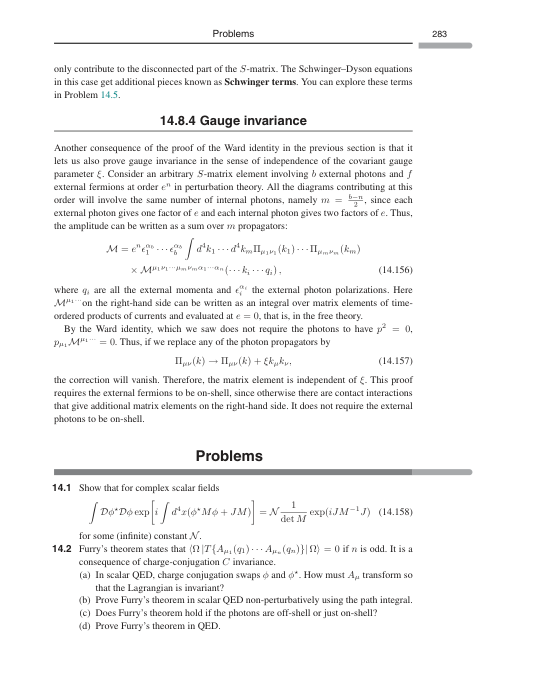
\includegraphics{./figs/14_Path_integrals_page_303.png}

---

